\subsubsection*{10.a}
On donne le droit de créer des indexes et selectionner la table DBAIOT.SERVICE a admin depuis DBAIOT

\lstinputlisting[style=sqlstyle]{SQL/Partie4/grant3.sql}

\begin{center}
    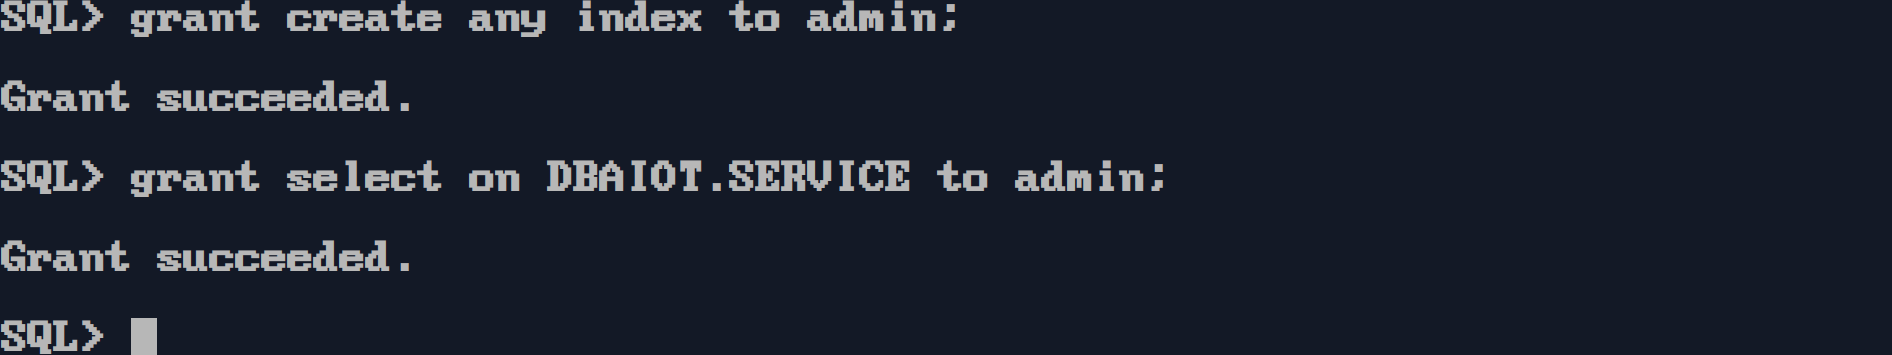
\includegraphics[width=\textwidth]{ScreenShot/Partie4/grant3.png}
\end{center}

\subsubsection*{10.b}
Creation de l'index NAMESERVICE\_IX depuis admin

\lstinputlisting[style=sqlstyle]{SQL/Partie4/index.sql}

\begin{center}
    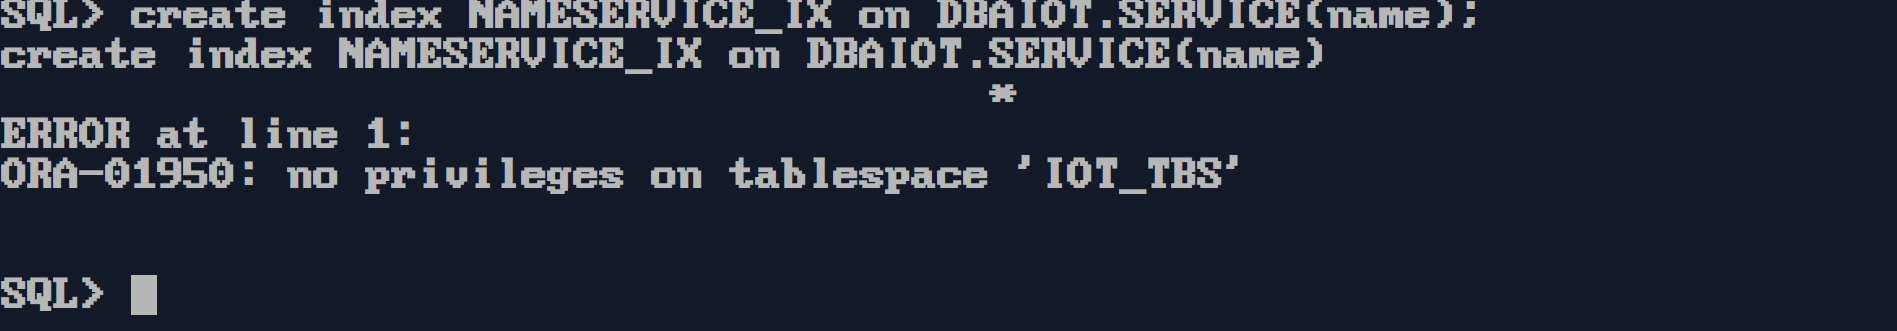
\includegraphics[width=\textwidth]{ScreenShot/Partie4/index1.png}
\end{center}

\begin{prettyBox}{Remarque}{myblue}
\begin{itemize}
\item Admin ne peut pas creer l'index NAMESERVICE\_IX puisqu'il n'a pas les privileges pour ecrire sur la tablespace IOT\_TBS 
\item Admin a pu creer la vue externe USER\_THING car les views externes sont stockes dans la tablespace system
\end{itemize}
\end{prettyBox}

